\documentclass{article}

% if you need to pass options to natbib, use, e.g.:
%     \PassOptionsToPackage{numbers, compress}{natbib}
% before loading neurips_2020

% ready for submission
% \usepackage{neurips_2020}

% to compile a preprint version, e.g., for submission to arXiv, add add the
% [preprint] option:
    \usepackage[preprint]{neurips_2020}

% to compile a camera-ready version, add the [final] option, e.g.:
    % \usepackage[final]{neurips_2020}

% to avoid loading the natbib package, add option nonatbib:
     % \usepackage[nonatbib]{neurips_2020}

\usepackage[utf8]{inputenc} % allow utf-8 input
\usepackage[T1]{fontenc}    % use 8-bit T1 fonts
\usepackage{hyperref}       % hyperlinks
\usepackage{url}            % simple URL typesetting
\usepackage{booktabs}       % professional-quality tables
\usepackage{amsfonts}       % blackboard math symbols
\usepackage{nicefrac}       % compact symbols for 1/2, etc.
\usepackage{microtype}      % microtypography
\usepackage{amsmath}        % math notation etc
\usepackage{graphicx}       % inserting images
\usepackage{float}          % image placement
\usepackage{array}          % table alignment
\usepackage{xcolor}         % to do macro

\newcommand{\R}{\mathbb{R}}
\newcommand{\bx}{\boldsymbol{x}}
\newcommand{\todo}[1]{\textcolor{red}{#1}}

\graphicspath{ {./figures/} }

\title{On Gaussian Processes for Regression}

% The \author macro works with any number of authors. There are two commands
% used to separate the names and addresses of multiple authors: \And and \AND.
%
% Using \And between authors leaves it to LaTeX to determine where to break the
% lines. Using \AND forces a line break at that point. So, if LaTeX puts 3 of 4
% authors names on the first line, and the last on the second line, try using
% \AND instead of \And before the third author name.

\author{
  Jeffrey Alido \\
  Department of Electrical and Computer Engineering \\
  Boston University \\
  \texttt{jalido@bu.edu} \\
  \And
  Shashank Manjunath \\
  Department of Electrical and Computer Engineering \\
  Boston University \\
  \texttt{manjuns@bu.edu} \\
}

\begin{document}

\maketitle

\author

\begin{abstract}
Gaussian processes emerged in machine learning as a powerful tool for regression and classification that provides
interpretability through kernel choice and uncertainty quantification. By leveraging properties of multivariate normal
distributions and Bayes’s rule, we may infer a probability distribution over possible functions when fitting a dataset.
This Bayesian framework allows flexibility through choosing a covariance function as a prior belief about the dataset,
which can provide further insight into the trends of the training data. We implement a multi-dimensional Gaussian
process regressor and evaluate its performance on the Boston Housing dataset, which is comparable to those in the top 25
of the Kaggle competition. Furthermore, we perform optimization on the hyperparameters through maximum likelihood
estimation, to remove the need for manual tuning of the hyperparameters.
\end{abstract}

\section{Gaussian Random Variables}

A random variable is a function that maps from an event space to a measurable space. The event space represents a set of
all possible outcomes that the random variable may take, and the measurable space is a probability measure between 0 and
1 (inclusive). We say that a random variable $X$ is normally distributed if the event space has a Gaussian probability
distribution, fully characterized by two parameters: a mean $\mu$ and variance $\sigma^2$:

\[
  X\sim \mathcal{N}(\mu,\sigma^2)
\]

For a one-dimensional Gaussian random variable, we refer to its distribution as a univariate Gaussian distribution. A
set of Gaussian random variables may be characterized jointly as a multivariate Gaussian distribution, with joint
probability distribution fully characterized by a mean vector and a covariance matrix:

\[
  X = \begin{bmatrix}
           X_{1} \\
           X_{2} \\
           \vdots \\
           X_{n}
         \end{bmatrix}   \sim \mathcal{N}(\boldsymbol{\mu},\Sigma)
\]

where $\boldsymbol{\mu}$ is the mean vector, and $\Sigma$ is the covariance matrix whose entries describe the covariance
between each pair of random variables.

\section{Gaussian Process}

A random process is essentially a collection of random variables jointly characterized  as a set or vector of random
variables with a multivariate joint probability distribution. A Gaussian process $f(\boldsymbol{x})$ is defined as a a
random process where each set of random variable in the random process is has a multivariate Gaussian distribution.
$f(\boldsymbol{x})$ is fully characterized by a mean function  $m(\boldsymbol{x})$ and covariance function,
$K(\boldsymbol{x},\boldsymbol{x'})$:

\[
  f(\boldsymbol{x})\sim\mathcal{GP}(m(\boldsymbol{x}),K(\boldsymbol{x},\boldsymbol{x'}))
\]

Typically, the mean function is zero. The kernel for the covariance is chosen based on some prior belief about the
dataset; more on kernels is discussed in \ref{subsection:kernels}.

\section{Regression}

Suppose we observe training data $\boldsymbol{t}$ and choose kernel $\kappa$. Then the mean and covariance functions are
given by 

\begin{gather*}
  m(\boldsymbol{x})=C_{\boldsymbol{x}\boldsymbol{t}}^\top C_{\boldsymbol{t}}^{-1}\boldsymbol{t} \\
  K(\boldsymbol{x},\boldsymbol{x'})=C_{\boldsymbol{x}\boldsymbol{x'}}-C_{\boldsymbol{x}\boldsymbol{t}}^\top
  C_{\boldsymbol{t}}^{-1}C_{\boldsymbol{x}\boldsymbol{t}}
\end{gather*}

where $C_{\boldsymbol{x}\boldsymbol{t}} = \kappa(\boldsymbol{x},\boldsymbol{t})$, $C_{\boldsymbol{t}} =
\kappa(\boldsymbol{t},\boldsymbol{t})$, and $C_{\boldsymbol{x}\boldsymbol{x'}} =
\kappa(\boldsymbol{x},\boldsymbol{x'})$.  Those interested in the derivation of the results are encouraged to consult
section 6.4.2 of \cite{bishop_pattern_2006}.

\subsection{Kernels} \label{subsection:kernels}

Covariance Functions or kernels, denoted $\kappa(\bx, \bx')$, form the core of a Gaussian process. Kernels allow
projection of input data into an alternate feature space, allowing easier separability of data in this new feature
space. Gaussian processes leverage kernels to featurize input data. In particular, if we have a function
$\Phi(\bx): \R^d \rightarrow \R^n$, we can write the kernel defined by this function as:

\[
  \kappa(\bx, \bx') = \langle \Phi(\bx), \Phi(\bx') \rangle = \Phi(\bx)^\top \Phi(\bx')
\]

In order to illustrate how kernels fit into Gaussian Processes, we will 

\todo{finish derivation of kernel trick in GP}

We illustrate specific kernels that we used below. These kernels can additionally be combined through addition and
multiplication of the kernels together, though we do not explore this as part of this project.

\subsubsection{Radial Basis Function (RBF) Kernel}

The Radial Basis Function (RBF) Kernel, also known as the Squared Exponential Kernel, is given by:

\[
  \kappa_{RBF}(\bx, \bx') = \sigma^2 \exp\left( - \frac{\|\bx -\bx' \|_{2}^{2}}{2 \ell^2} \right)
\]

This kernel is parametrized by two parameters, the lengthscale $\ell$ and the variance $\sigma^2$. The lengthscale
determines the width of the kernel, and the variance scales the kernel\cite{duvenaud_automatic_2014}. We provide an
images of the RBF Kernel with various lengthscales and variances in Figure~\ref{fig:square_exp_kernel}

\subsubsection{Rational Quadratic Kernel}

The Rational Quadratic Kernel is another standard kernel is similar to the RBF kernel. It can be constructed from
summing RBF kernels with varying lengthscales. The kernel is given by:

\[
  \kappa_{RQ}(\bx, \bx') = \sigma^2 \left( 1 + \frac{\| \bx - \bx' \|_{2}^{2}}{2 \alpha \ell^2} \right)^{-\alpha}
\]

This kernel is parametrized by three parameters, the lengthscale $\ell$, the variance $\sigma^2$, and the lengthscale
weighting parameter $\alpha$\cite{duvenaud_automatic_2014}. We provide images of the Rational Quadratic Kernel with
various $\alpha$ values in Figure~\ref{fig:rqk}

\subsubsection{Periodic Kernel}

The periodic kernel allows us to model periodic functions. The kernel is given by:

\[
  \kappa_{P}(\bx, \bx') = \sigma^{2}  \exp(- \frac{2 \sin^{2}(\pi \|\bx - \bx'\|)}{p \ell^{2}})
\]

This kernel is parametrized by two parameters, $p$ which describes the period of the function, and $\ell$ which is the
lengthscale\cite{duvenaud_automatic_2014}. We provide images of the Periodic Kernel with various $p$ values in
Figure~\ref{fig:periodic_kernel}


\section{A Simple Demo}

\todo{fit some GPs on sine waves or something}

\section{Boston Housing Dataset}

The Boston Housing Dataset, originally published in 1978 contains 506 data points, each containing 13 features and 1
label for regression\cite{harrison_hedonic_1978}. The dataset provides the median value of houses in Boston suburbs.
This dataset is particularly suitable for Gaussian processes, as the dataset is quite small. Use of Gaussian processes
allows us to accurately quantify our uncertainty for each The label is the median value of owner-occupied homes in \$1000s, and
all other features are used for model fitting. The features included in the dataset are given in the table in Table
\ref{table:bhd_feat}.

\begin{table}[H]
  \centering
  \caption{Table of Boston Housing Dataset feature names and features}
  \begin{tabular}{ || m{3cm} | m{7cm} || }
    \hline
    \textbf{Feature Name} & \textbf{Feature Description} \\
    \hline \hline
    CRIM    & Per capita crime rate by town \\
    \hline
    ZN      & Proportion of residential land zoned for lots over 25,000 sq.ft. \\
    \hline
    INDUS   & Proportion of non-retail business acres per town. \\
    \hline
    CHAS    & Charles River dummy variable (1 if tract bounds river; 0 otherwise) \\
    \hline
    NOX     & Nitric oxides concentration (parts per 10 million) \\
    \hline
    RM      & Average number of rooms per dwelling \\
    \hline
    AGE     & Proportion of owner-occupied units built prior to 1940 \\
    \hline
    DIS     & Weighted distances to five Boston employment centres \\
    \hline
    RAD     & Index of accessibility to radial highways \\
    \hline
    TAX     & Full-value property-tax rate per \$10,000 \\
    \hline
    PTRATIO & Pupil-teacher ratio by town \\
    \hline
    B       & $1000(Bk - 0.63)^2$ where Bk is the proportion of Black people by town \\
    \hline
    LSTAT   & \% lower status of the population \\
    \hline
    MEDV    & Median value of owner-occupied homes in \$1000's \\
    \hline
  \end{tabular}
  \label{table:bhd_feat}
\end{table}

For the application of Gaussian Processes, we use the regression task, i.e. fitting to the MEDV feature. Prior to
fitting on the data, we normalize the data per feature. Specifically, for each feature in the dataset, we perform the
following operation:

\[
  X_{\text{feat}} = \frac{X_{\text{feat}} - \mu(X_{\text{feat}})}{\sigma(X_{\text{feat}})}
\]

where $\mu(X)$ is the mean value of that feature in the training set, and $\sigma(X)$ is the standard deviation of that
feature in the training set. We additionally normalize the MEDV feature, and convert it back to non-normalized units
before calculating our RMSE.

\section{Results}
\section{Figures}
\begin{figure}[H]
  \centering
  \caption{Graph of a square exponential kernel for various lengthscales and variances}
  \label{fig:square_exp_kernel}
  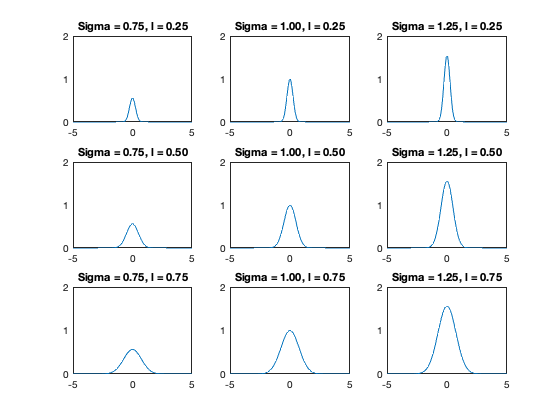
\includegraphics[trim={0 7cm 0 7cm},clip,keepaspectratio=true,scale=0.5]{square_exp_kernel}
\end{figure}
\begin{figure}[H]
  \centering
  \caption{Graph of a rational quadratic kernel for $\sigma = 1$, $\ell = 1$, and various $\alpha$ values}
  \label{fig:rqk}
  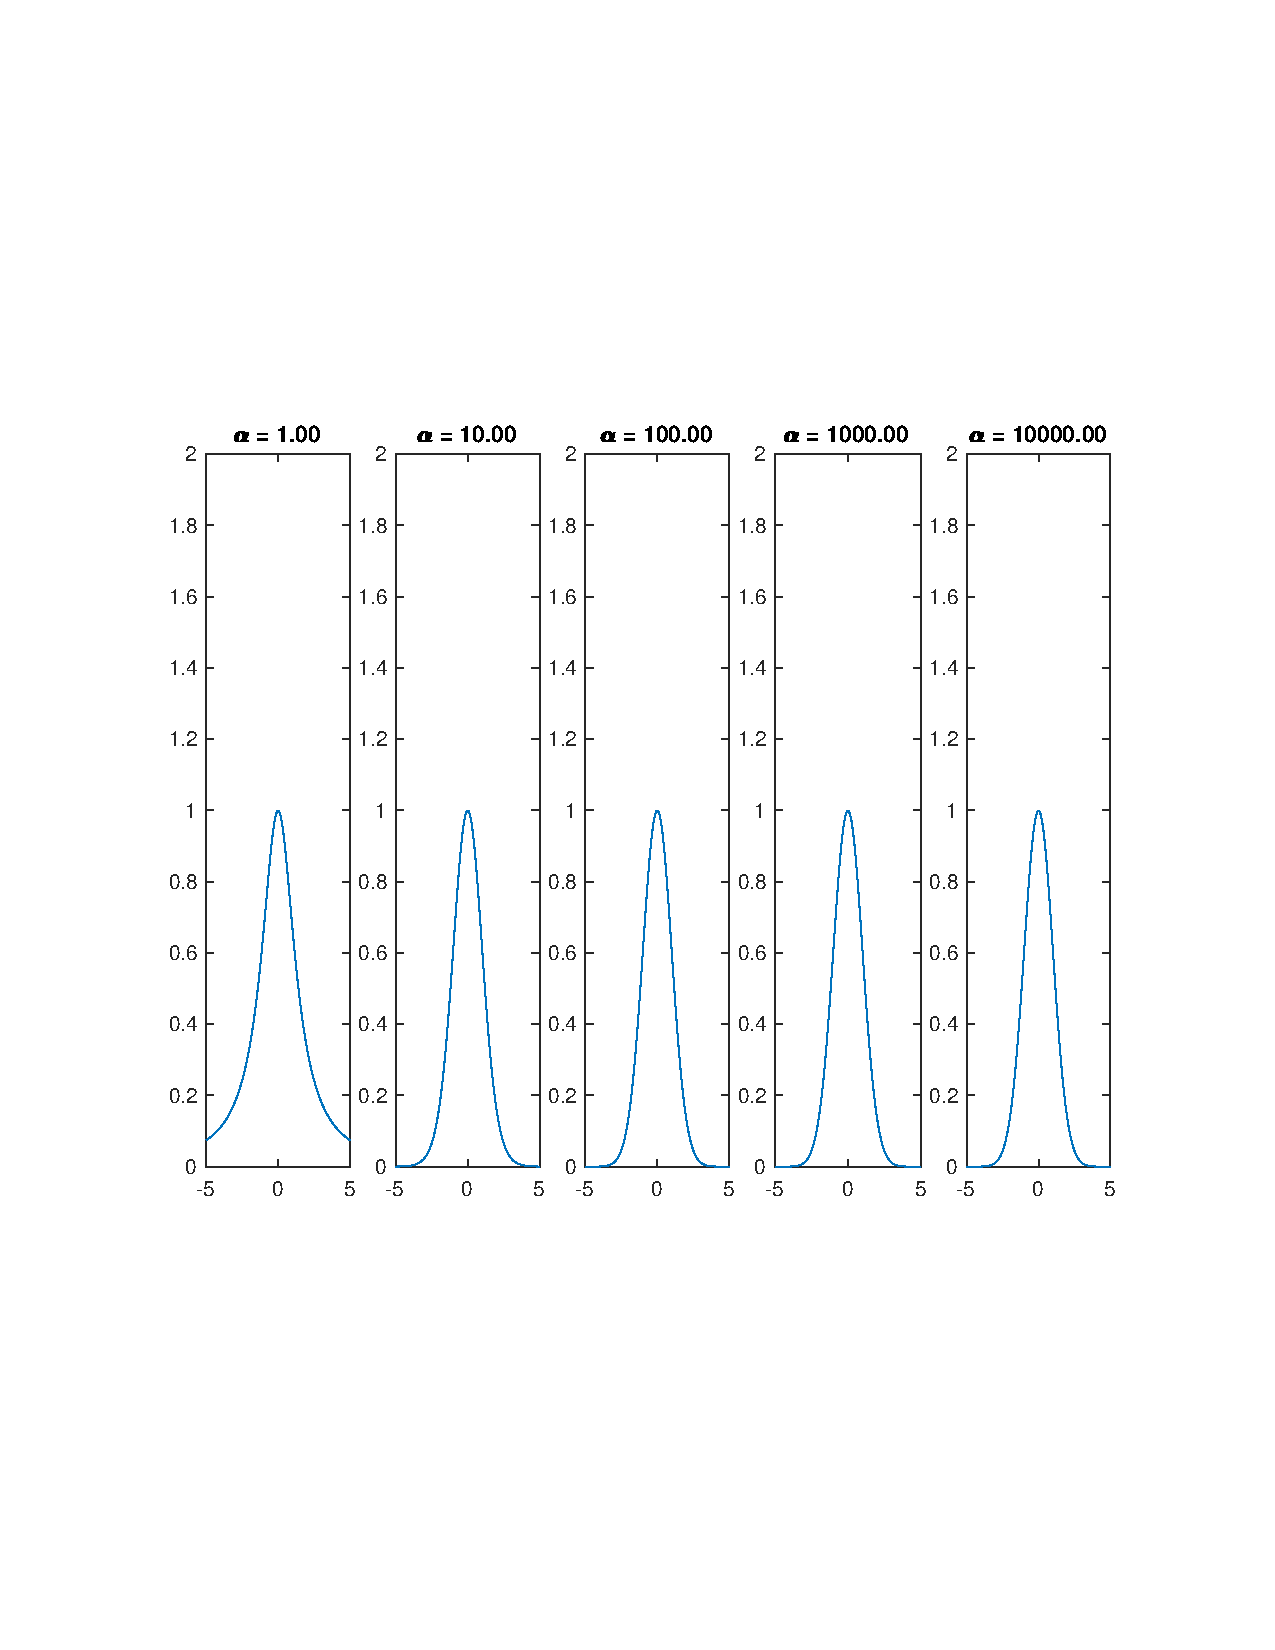
\includegraphics[trim={0 7cm 0 7cm},clip,keepaspectratio=true,scale=0.5]{rqk}
\end{figure}
\begin{figure}[H]
  \centering
  \caption{Graph of a rational quadratic kernel for $\sigma = 1$, $\ell = 1$, and various $p$ values}
  \label{fig:periodic_kernel}
  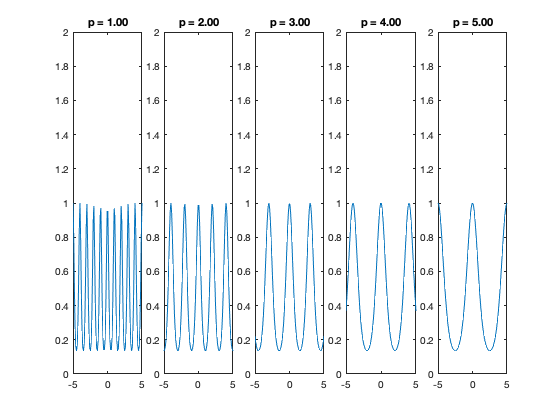
\includegraphics[trim={0 7cm 0 7cm},clip,keepaspectratio=true,scale=0.5]{periodic_kernel}
\end{figure}

\section{References}
\bibliographystyle{plain}
\bibliography{gpr}

\end{document}
